\documentclass[a4paper]{article}
\usepackage[spanish]{babel}
\usepackage[utf8]{inputenc}
\usepackage{amsmath}
\usepackage{listings}
\usepackage{xcolor}
\usepackage{amsfonts}
\usepackage{amssymb}
\usepackage[pdftex]{hyperref}
\usepackage{todonotes}
\usepackage{graphicx}

\begin{document}
    \title{\textbf{Proyecto \#1 DAA:} Procastinaci\'on ++}
    \author{L\'azaro Daniel Gonz\'alez Mart\'inez y Alejandra Monz\'on Pe\~na}
    \date{}
    \maketitle

    \section*{Desccripci\'on del problema}
    Sean las cadenas \textbf{S}, \textbf{T} y una cadena vac\'ia \textbf{A}, se construyen nuevas cadenas de la siguiente forma: 

    \begin{itemize}
        \item[$\diamond $] Quitar la primera letra de \textbf{S} y ponerla al inicio de la cadena \textbf{A}.
        \item[$\diamond $] Quitar la primera letra de \textbf{S} y ponerla al final de la cadena \textbf{A}.    
    \end{itemize}

    Estas operaciones se pueden realizar hasta que \textbf{S} quede sin caracteres.\\ 

    Se desea contar cuántas cadenas diferentes se pueden crear con estas operaciones tales que \textbf{T} sea prefijo de 
    la nueva cadena (\textbf{A}).\\ 

    Definimos por comodidad la construcci\'on de cadenas combinando de cualquier forma posible las dos operaciones permitidas como 
    \textit{construcci\'on por aburrimiento}.

    \section*{Soluci\'on Backtrack}
    Una primera soluci\'on al problema planteado se puede obtener haciendo una exploraci\'on por todas las posibles cadenas que se pueden formar 
    y en cada caso comprobar si \textbf{T} es prefijo de dicha cadena. 

    		% Configuración de Listings
	\lstset{keywordstyle=\color{blue}, basicstyle=\small}

	\begin{figure}[htb]
	
    \begin{lstlisting}[language=Python]

        def Procastinacion(S,T):
            if len(T) > len(S):
                return 0
            return Procastinacion2(S,T,'',0)
        
        def Procastinacion2(S,T,A,i):
            m = len(T)
            k = len(A)
            if len(S) <= i:
                return T == A[0:m]
            return Procastinacion2(S,T,f'{A}{S[i]}',i+1) 
                        + Procastinacion2(S,T,f'{S[i]}{A}',i+1) 
                            + ((m <= k) and (T == A[0:m]))
	\end{lstlisting}
	\caption{Código python del backtrack.}
	\end{figure}

    Este algoritmo de soluci\'on, aunque efectivo es demasiado costoso computacionalmente, sean $|S| = n$ y $|T| = m$, se tiene que:

    \begin{equation*}
        T(n,m) = 2 T(n-1) + m 
    \end{equation*}

    de donde, al utilizar el Teorema Maestro para funciones decrecientes, se obtiene para este problema que 
     $T(n,m) = \Theta(2^n + m)$.

    \section*{Explotando caracter\'isticas del problema}
    Una primera mejora que se puede hacer, se basa en la idea de que la primera letra de \textbf{S} 
    al poder colocarse tanto al inicio como al final de la cadena vac\'ia \textbf{A}, se generan así dos \'arboles de cadenas exactamente iguales (con las mismas cadenas), solo que estas se pueden considerar ``diferentes'' por 
    haber tenido una decisi\'on inicial distinta.\\ 

    Por tanto una mejora inicial, consiste en no duplicar innecesariamente el espacio de b\'usqueda, sino asumir que en \textbf{A} inicialmente 
    est\'a el primer caracter de \textbf{S} y duplicar el resultado final. Aunque esta idea no mejora la complejidad temporal, reduce a la mitad la cantidad de operaciones a realizar.

    \section*{Soluci\'on con Programaci\'on Din\'amica}

    Representando las cadenas \textbf{S} y \textbf{T} por sus caracteres, tenemos:

    \begin{itemize}
        \item[] \textbf{T} = $T_0T_1 ... T_{m-1}$
        \item[] \textbf{S} = $S_0S_1 ... T_{n-1}$ 
    \end{itemize}

    Entonces $T_i$ ($S_i$) denota al i-\'esimo m\'as un cararacter de \textbf{T}(\textbf{S}), de igual modo 
    $T_{i...j}$($S_{i...j}$) denota a la subcadena $T_iT_{i+1}...T_j$ ($S_iS_{i+1}...S_{j}$) de la cadena \textbf{T} (\textbf{S}).\\
    
    Definamos la funci\'on $f(i,j)$ como la cantidad de cadenas $A_{i...j}$ \textit{construidas por aburrimiento} con los primeros $j-i+1$ 
    caracteres de S (es decir con los caracteres de $S_{0...j-i}$) donde 
    para:
    \begin{itemize}
    	\item[i] $j < m$, $\quad A_{i...j} = T_{i...j}$
    	\item[ii] $j \geq m $ y $i < m $, $\quad A_{i...j} = T_{i...m-1}A_{m...j}$
    	\item[iii] $i > m $, $\quad A_{i...j} = A_{i...j}$
    \end{itemize}
    
    Luego $\sum_{j= m-1}^{n-1}f(0,j)$ es la cantidad total de cadenas que se pueden \textit{construir por aburrimiento} que tienen como prefijo a \textbf{T}.\\
    
    Notemos qu\'e, para $i < m$ se cumple que: %TODO:

    \begin{equation}\label{eq:1}
        f(i,i) = \left\{ \begin{aligned}
            &2, &T_i = S_0\\
            &0, &eoc
        \end{aligned} \right.
    \end{equation}

    Esto se debe a que, como queremos formar subcadenas de tama\~no 1 de \textbf{T} con el primer caracter de \textbf{S}, tenemos en los casos que hay coincidencia (\ref{fig:ppp1}), dos maneras de colocar el caracter, (por delante y por detr\'as) y en los restantes casos 
    se tiene 0 puesto que no se tiene ninguna subcadena de \textbf{T} de longitud 1 al tomar ese caracter (\ref{fig:ppp0}).\\
        
    \begin{figure}[!h]
    	\centering
    	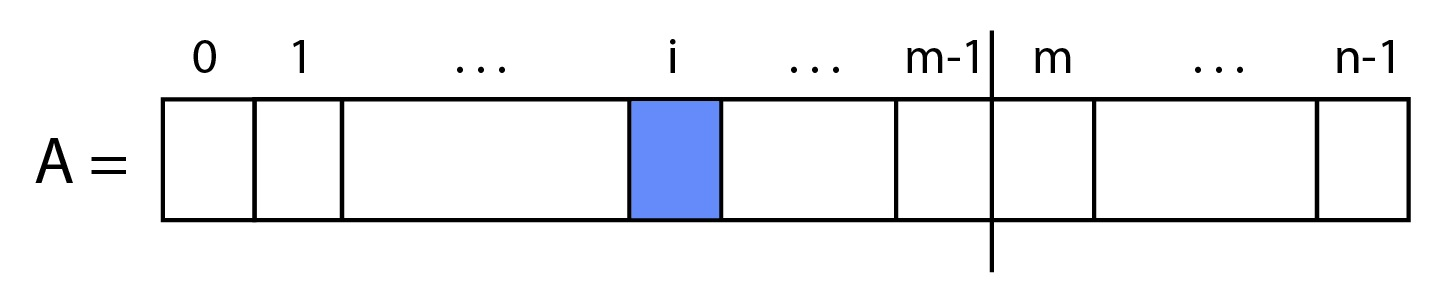
\includegraphics[width=0.7\linewidth]{ppp1}
    	\caption{Formas de colocar el $0-$ésimo caracter de $S$ en la posición $i-$ésima de $A$ (por la derecha y por la izquierda) cuando hay coincidencia y $i<m$.}
    	\label{fig:ppp1}
    \end{figure}

	\begin{figure}[!h]
		\centering
		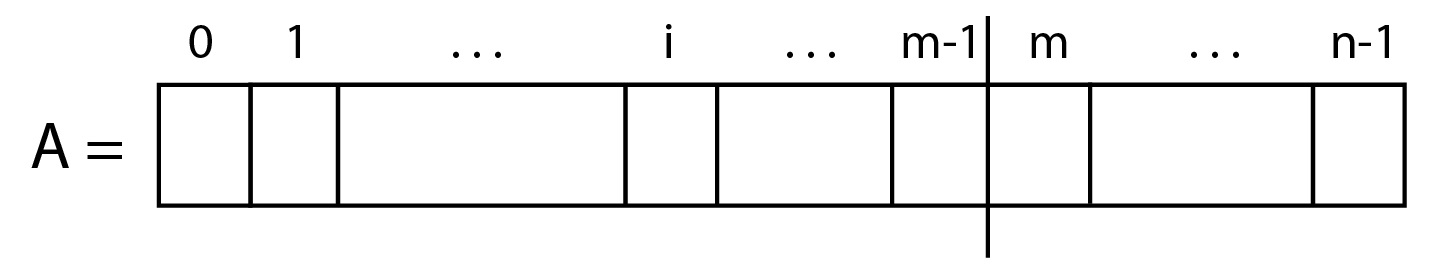
\includegraphics[width=0.7\linewidth]{ppp0}
		\caption{Formas de colocar el $0-$ésimo caracter de $S$ en la posición $i-$ésima de $A$ (no hay forma) cuando no hay coincidencia y $i<m$.}
		\label{fig:ppp0}
	\end{figure}

    
    
    Adem\'as se cumple, para $i \geq m$, que $f(i,i) = 2$, puesto que poner cualquier caracter en posiciones de \textbf{A} mayores que el prefijo $T$ (\ref{fig:ppp2}) origina una cadena de longitud 1 válida para la definición de la función $f$ (iii) y el valor es 2, puesto que de igual modo este caracter se pudo colocar por delante o por atrás de la cadena vacía.\\
    
    \begin{figure}[!h]
    	\centering
    	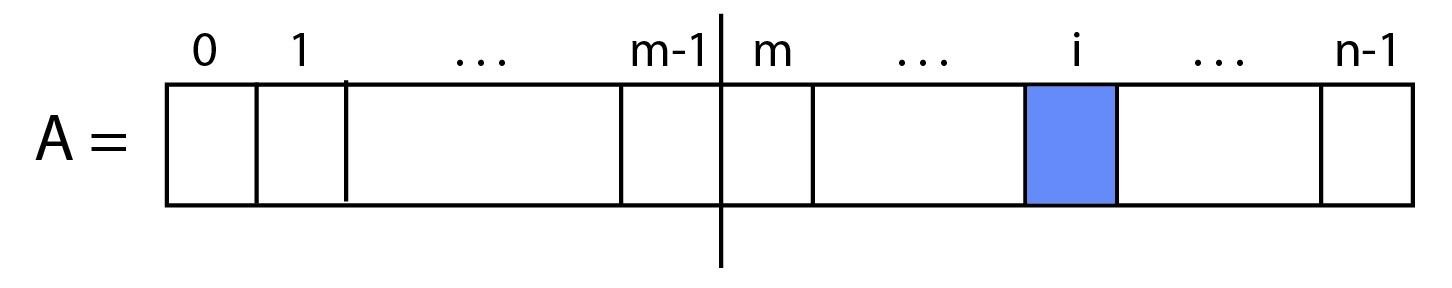
\includegraphics[width=0.7\linewidth]{ppp2}
    	\caption{Formas de colocar el $0-$ésimo caracter de $S$ en la posición $i-$ésima de $A$ (por la derecha y por la izquierda) cuando $i \ge m$.}
    	\label{fig:ppp2}
    \end{figure}
     

    A modo general $f(i,j)$ se puede construir recursivamente como: 

    \begin{equation*}
        f(i,j) = f(i+1,j)\mathbb{I}_{ \{T_i = S_{j-i+1} \vee i \geq m \}}  +  f(i,j-1)\mathbb{I}_{ \{T_j = S_{j-i+1} \vee j \geq m \} } 
    \end{equation*}

    Ya que $S_{j-i+1}$ se puede agregar por delante a las cadenas $A_{i+1}...A_j$ (\ref{fig:ppp3}), o por atr\'as a las cadenas 
    $A_{i}...A_{j-1}$ (\ref{fig:ppp4}), cuando $S_{j-i+1}$ coincide con $T_i$ o $T_j$ respectivamente, formando as\'i cadenas $A_{i}...A_{j}$.\\
    
    \begin{figure}[h!]
    	\centering
    	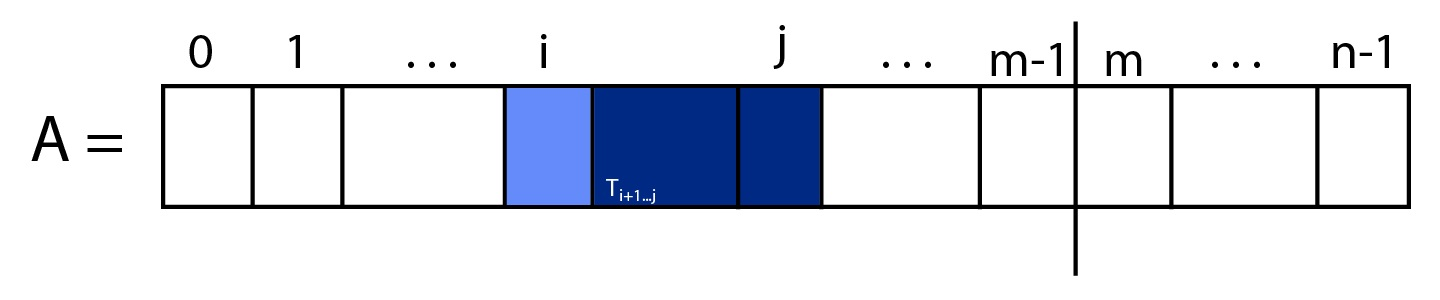
\includegraphics[width=0.7\linewidth]{ppp3}
    	\caption{Forma de colocar el $(j-i+1)-$ésimo caracter de $S$ en la posición $i-$ésima de $A$ (por la izquierda) cuando $j < m$, solo cuando hay coincidencia.}
    	\label{fig:ppp3}
    \end{figure}
    \begin{figure}[h!]
    	\centering
    	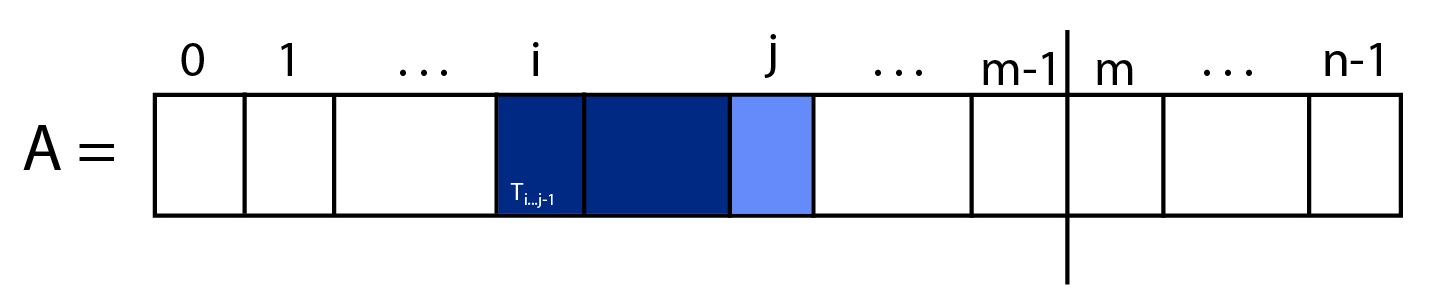
\includegraphics[width=0.7\linewidth]{ppp4}
    	\caption{Forma de colocar el $(j-i+1)-$ésimo caracter de $S$ en la posición $j-$ésima de $A$ (por la derecha) cuando $j < m$, solo cuando hay coincidencia.}
    	\label{fig:ppp4}
    \end{figure}
    

    En los casos (ii), a la subcadena $A_{i...j-1}$ se le puede agregar el caracter $S_{j-i+1}$ por atr\'as sin afectar 
    el prefijo (\ref{fig:ppp5a}), generando la cantidad de cadenas que hab\'ia en $f(i,j-1)$, pero ahora de la forma $A_{i...j}$. Note que esta condición no implica que no se pueda cumplir que $T_{i} =  S_{j-i+1}$ por lo que en este caso podría ponerse por delante sin problema (\ref{fig:ppp5}).\\
    
    \begin{figure}[h!]
    	\centering
    	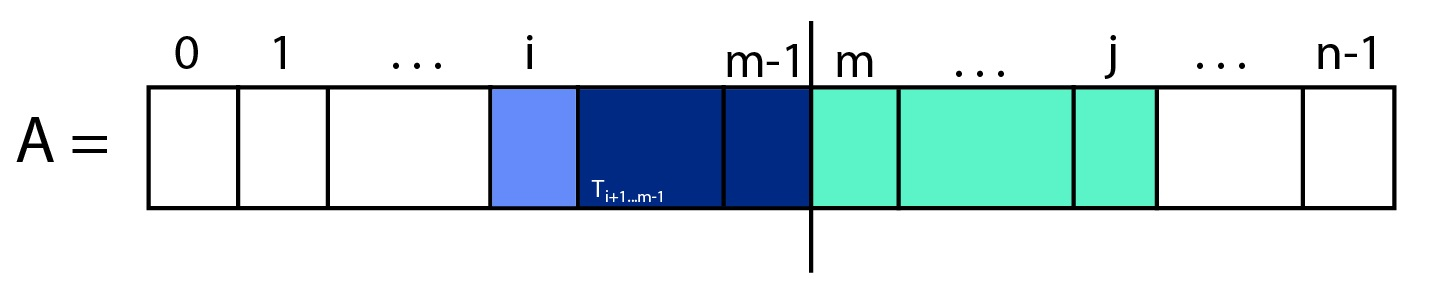
\includegraphics[width=0.7\linewidth]{ppp5}
    	\caption{Forma de colocar el $(j-i+1)-$ésimo caracter de $S$ en la posición $i-$ésima de $A$ (por la izquierda) cuando $i < m$ y $j > m$, solo cuando hay coincidencia}
    	\label{fig:ppp5a}
    \end{figure}

	\begin{figure}[h!]
		\centering
		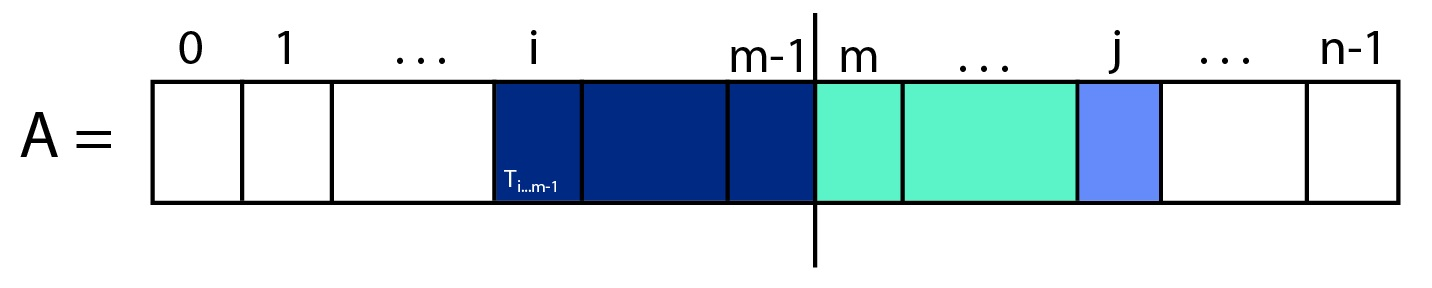
\includegraphics[width=0.7\linewidth]{ppp5a}
		\caption{Forma de colocar el $(j-i+1)-$ésimo caracter de $S$ en la posición $j-$ésima de $A$ (por la derecha) cuando $i < m$ y $j \ge m$, sin importar la coincidencia.}
		\label{fig:ppp5}
	\end{figure}
    
    
    Por \'ultimo cuando $i \geq m$ entonces $j \geq m$ y se puede agregar $S_{j-i+1}$ como prefijo de 
    $A_{i+1...j}$ (\ref{fig:ppp6}) y como sufijo de $A_{i...j-1}$ (\ref{fig:ppp7}) cayendo en el caso (iii), por lo tanto tendr\'iamos $f(i+1,j) + f(i,j-1)$ cadenas de la forma $A_{i...j}$.
    
    \begin{figure}[h!]
    	\centering
    	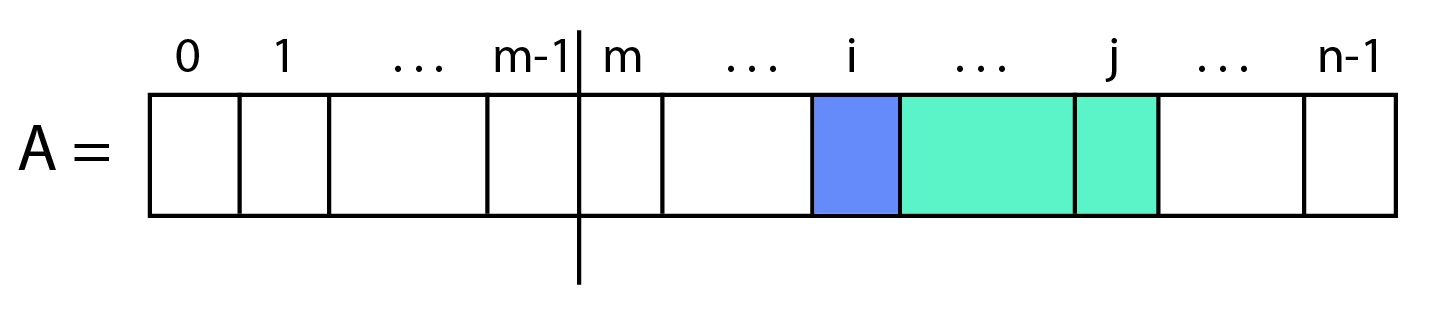
\includegraphics[width=0.7\linewidth]{ppp6}
    	\caption{Forma de colocar el $(j-i+1)-$ésimo caracter de $S$ en la posición $i-$ésima de $A$ (por la izquierda) cuando $i \ge m$, sin importar coincidencia.}
    	\label{fig:ppp6}
    \end{figure}
    \begin{figure}[h!]
    	\centering
    	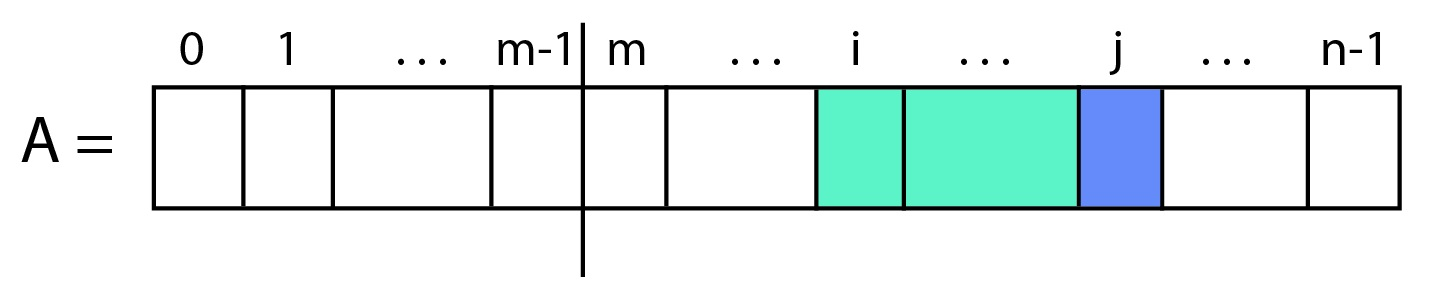
\includegraphics[width=0.7\linewidth]{ppp7}
    	\caption{Forma de colocar el $(j-i+1)-$ésimo caracter de $S$ en la posición $j-$ésima de $A$ (por la derecha) cuando $i \ge m$, sin importar coincidencia.}
    	\label{fig:ppp7}
    \end{figure}

\section*{Implementación de la dinámica}
    
    
    \begin{lstlisting}[language=Python]
def solve_dp(S,T):
    n = len(S)
    m = len(T)
        
    if m > n:
        return 0
        
    dp = [[0 for j in range(n)] for i in range(n)]
    
    for i in range(n):
        if i >= m or T[i] == S[0]:
            dp[i][i] = 2
    
    for k in range(1, n):    
        c = S[k]
        
        i = 0        
        for j in range(k, n):
            if i >= m or c == T[i]:
                dp[i][j] += dp[i+1][j]
            if j >= m or c == T[j]:
                dp[i][j] += dp[i][j-1]            
            i += 1            
    
    return sum(dp[0][m-1:])
    \end{lstlisting}
	
	\section*{Correctitud del algoritmo}
	
	Como nos queda claro que $\sum_{j= m-1}^{n-1}f(0,j)$ es la respuesta a nuestro problema, demostrar que $dp[i][j] = f(i,j)$, sería suficiente para probar la correctitud del algoritmo. Por lo tanto demostremos que en el momento que se actualiza el valor de $dp[i][j]$ este coincidirá con $f(i,j)$.
	
	Hagamos inducción en la longitud de la cadena que estamos formando $A_{i...j}$, lo que es equivalente a hacer la inducción sobre el ciclo en que itera $k$.
	
	\begin{itemize}
		\item Caso base: $|A_{i...j}| = 1$
		
		Como por definición, $i \leq j$ entonces $|A_{i...j}| = 1$ si y solo si $i = j$, ya que $|A_{i...j}| = j-i + 1 = 1$.
		Luego todas las cadenas que puedan pertenecer a nuestro caso base están en la diagonal de $dp$, y se inicializan atendiendo a la definición de $f(i, i)$ dada en (\ref{eq:1}), entonces tenemos que:
		$$dp[i][i] = f(i, i)$$.
		Note que se inicializan así en el ciclo que itera por $i$ del código.
		
		\item Caso Hipótesis: Supongamos que para toda cadena $A_{i^\prime...j^\prime}$ de tamaño menor que $p$ se cumple que $dp[i^\prime][j^\prime] = f(i^\prime, j^\prime)$ con $j^\prime - i^\prime + 1 < p$. Esto es equivalente a que hasta la iteración $p-1$ del ciclo que itera sobre $k$, se cumple que lo planteado anteriormente\footnote{Observe que, para que la fórmula tenga sentido, $i^\prime \leq j^\prime$}.
		
		Sea $A_{i...j}$ de tamaño $p$. Podemos asumir $i<j$, porque el caso base ya está tratado a parte. Luego como
		$$f(i,j) = f(i+1,j)\mathbb{I}_{ \{T_i = S_{j-i+1} \vee i \geq m \}}  +  f(i,j-1)\mathbb{I}_{ \{T_j = S_{j-i+1} \vee j \geq m \} } $$
		se aprecia que $f(i,j)$ depende de los valores de $f(i+1,j)$ y $f(i,j-1)$. Luego como $|A_{i+1...j}| = j-(i+1) + 1 = j-i$, y $j-i < p$, entonces por hipótesis $f(i+1,j) = dp[i+1][j]$. De manera similar como $|A_{i...j-1}| = j-1 - i + 1 = j-i < p$, aplicamos la hipótesis pero en este caso $f(i,j-1) = dp[i][j-1]$.
		Luego
		$$f(i,j) = dp[i+1][j]\mathbb{I}_{ \{T_i = S_{j-i+1} \vee i \geq m \}}  +  dp[i][j-1]\mathbb{I}_{ \{T_j = S_{j-i+1} \vee j \geq m \} } $$
		y finalmente $dp[i][j]$ al actualizarse con este cálculo nos quedará:
		$$dp[i][j] = f(i,j)$$				
	\end{itemize}

	Luego por Principio de Inducción Matemática demostramos que al concluir el algoritmo queda computado para cada $dp[i][j]$, con $0 \leq i\leq j < n$, la cantidad de cadenas $A_{i...j}$ que se pueden \textit{construir por aburrimiento} con los primeros $|A_{i...j}| = j-i+1$ caracteres de $S$, es decir, queda guardado en $dp[i][j]$ el valor de $f(i,j)$.	
	
	\section*{Complejidad Temporal}
	
	Definir e inicializar la matriz $dp$ se hace en $2n^2$ operaciones ya que esta tiene dimensión $n \times n$.
	
	El ciclo que itera por $k$ ejecuta el ciclo que itera por $j$, unas $n-1$ veces. Y este ciclo se ejecuta $n-k$ veces para la iteración $k$. Es decir, ambos ciclos ejecutan un total de veces igual a:
	$$ \sum_{k=1}^{n-1} (n-k) = (n-1) + (n-2) + ... + 1 = \frac{n(n-1)}{2} $$
	
	Finalmente cuando se calcula la suma de los $dp[0][i]$ para $i \geq m$, se hacen $n-m + 1$ iteraciones.
	
	Por lo tanto al sumar cada uno de estos costos considerando también, el tiempo constante que requieren las operaciones intermedias, nos quedaría algo así:
	
	$$T(n,m) = c_1 + 2n^2 + c_2\frac{n(n-1)}{2} + n-m+1$$
	
	Demostremos que $T(n,m)$ es $O(n^2)$:
	
	Para esto debemos encontrar una constante $C$ tal que a partir de cierto $n$, se cumpla $T(n,m) \leq Cn^2$.
	$$T(n,m) \leq c_1 + 2n^2 + c_2\frac{n(n-1)}{2} + n + 1$$
	
	Calculemos el límite:
	$$ \lim_{n}\left(\frac{c_1 + 2n^2 + c_2\frac{n(n-1)}{2} + n + 1}{n^2}\right)$$
	$$= \lim_{n}\left(\frac{2c_1 + 4n^2 + c_2n(n-1) + 2n + 2}{2n^2}\right)$$
	$$= \frac{4+c_2}{2}$$
	Como este límite es finito y mayor que $0$, existirá una constante $C$ tal que :
	$$ c_1 + 2n^2 + c_2\frac{n(n-1)}{2} + n + 1 \leq Cn^2$$
	y por transitividad, $ T(n,m) \leq Cn^2 $. Luego $T(n,m)$ es $O(n^2)$.
	
	Incluso si queremos ser más exquisitos podemos demostrar que $T(n,m) = \theta(n^2)$. \\
	
	Como:
	$$c_1 + 2n^2 + c_2\frac{n(n-1)}{2} \leq T(n,m)$$
	Calculando el límite siguiente:
	$$ \lim_{n}\left(\frac{c_1 + 2n^2 + c_2\frac{n(n-1)}{2}}{n^2}\right)$$
	$$= \lim_{n}\left(\frac{2c_1 + 4n^2 + c_2n(n-1)}{2n^2}\right)$$
	$$= \frac{4+c_2}{2}$$
	De forma similar, existirá una constante $C$ tal que a partir de cierto $n$, se cumple que 
	$$Cn^2 \leq c_1 + 2n^2 + c_2\frac{n(n-1)}{2}$$
	y por transitividad se cumple que $Cn^2 \leq T(n,m)$. Luego $T(n,m) = \Omega(n^2)$. Y finalmente $T(n,m)$ es $\theta(n^2)$.
	
	\section*{Generador y Probador de casos}
	
	Para comprobar la correctitud y eficiencia de los algoritmos creamos un generador y probador de casos pruebas. Para la generación de casos definimos 3 alfabetos:
	\begin{itemize}
		\item $A_1 = \{\texttt{a},\texttt{b},\texttt{c}\}$
		\item $A_2 = \{\texttt{a},\texttt{b},\texttt{c},\texttt{d}\}$
		\item $A_3 = \{\texttt{a},\texttt{b},\texttt{c},\texttt{d},\texttt{e}\}$
	\end{itemize}

	Generamos $6$ cadenas $T$, con longitud entre $2$ y $19$. Y por cada $T$ se generaron cadenas $S$ de tamaño desde $|T|$ hasta $10|T|-1$, de $3$ tipos, mezclando aleatoriamente las letras de $T$ con las que se pueden añadir según el alfabeto del tipo seleccionado:
	\begin{itemize}
	\item Tipo 1: Añadiendo caracteres del Alfabeto 1
	\item Tipo 2: Añadiendo caracteres del Alfabeto 2
	\item Tipo 3: Añadiendo caracteres del Alfabeto 3
	\end{itemize}
	La selección aleatoria de los caracteres es uniforme, es decir, cada letra tiene la misma probabilidad de ser seleccionada.
	
	De esta forma se generaron $22680$ casos de pruebas de los que $7404$ resultaron con valor de $0$ al ser evaluadas por el algoritmo de programación dinámica, para representar el $32.6455\%$ de los casos totales. Para comparar ambos algoritmos, se utilizaron $630$ casos de pruebas de los que el $92$ de ellos resultaron en $0$, representando el $14.6031\%$ de estos. Además para los $630$ casos seleccionados, se obtuvo el mismo valor al evaluar ambos algoritmos. La diferencia significativa de ambos algoritmos es en la complejidad temporal, donde analíticamente son muy diferentes. Y en la práctica esto se comprobó donde, los $630$ casos corrieron en menos de $1$ minuto con el algoritmo de programación dinámica. Mientras que con el algoritmo de backtrack, se demoró más de $12$ horas.
	
	El generador, el tester, y el comparador se encuentran en los archivos \texttt{generator.py}, \texttt{tester.py} y \texttt{check.py}, respectivamente.


\end{document}